\chapter{Natural Gradient Descent}
\label{ch:natural_gradient}

% 1. Descriptive opening
Standard gradient descent has served as the undisputed workhorse for optimizing neural networks, dutifully updating parameters by taking steps in the direction of the steepest descent of the empirical loss landscape. However, this classical approach implicitly relies on a strong assumption about the geometry of the parameter space: it assumes that the space $\mathbb{R}^d$ is fundamentally flat and Euclidean. In a Euclidean geometry, a step of length $\epsilon$ in any direction is considered equal. But when training deep learning models—particularly probabilistic models—our primary object of interest is not the parameter vector $\theta$ itself, but rather the probability distribution $p_\theta(x)$ or the conditional distribution $p_\theta(y|x)$ that these parameters induce over the data. 

The mapping from the parameter space to the manifold of probability distributions is highly complex and non-linear. A small Euclidean change in the parameters might lead to an enormous change in the resulting distribution in one region of the parameter space, causing the model to completely forget its learned representations. Conversely, a massive change in parameters might leave the output distribution virtually untouched in another region, leading to agonizingly slow convergence. Standard gradient descent is blind to this underlying structure. It minimizes the loss function by traversing the parameter space blindly, often taking inefficient, oscillating paths because it misjudges the true "distance" it has traveled in terms of the model's predictive behavior.

Information geometry offers a profound shift in perspective. Instead of viewing optimization as a journey through a flat parameter space, we view it as navigating the curved \textit{statistical manifold} of probability distributions. In this Riemannian manifold, the distance between two nearby distributions is measured not by the Euclidean distance between their parameters, but by the Kullback-Leibler (KL) divergence, a fundamental measure of information loss. The Fisher Information Matrix (FIM), as introduced in Chapter 29, acts as the Riemannian metric tensor that precisely quantifies this local curvature.

Natural Gradient Descent (NGD), pioneered by Shun-ichi Amari, is the optimization algorithm designed explicitly to walk on this statistical manifold. By correcting the standard gradient with the inverse of the Fisher Information Matrix, NGD ensures that optimization steps are of constant size in the \textit{distributional} space, rather than the parameter space. This leads to a descent direction that is perfectly invariant to the parameterization of the model. Whether we parameterize a Gaussian distribution by its variance, its standard deviation, or its precision, the natural gradient yields the exact same sequence of distributions during optimization. This chapter delves into the mathematical formulation of the natural gradient, proving its status as the steepest descent direction in probability space, illustrating its mechanical advantages, and exploring its implications for modern deep learning.

% 2. Mathematical core
\section{The Geometry of Steepest Descent}

To rigorously derive Natural Gradient Descent, we first revisit standard gradient descent from a variational perspective. Suppose we have a loss function $\mathcal{L}(\theta)$ that we wish to minimize. Standard gradient descent updates $\theta$ to $\theta + \Delta \theta$ by finding the direction $\Delta \theta$ that minimizes the first-order Taylor expansion of the loss, subject to a constraint on the step size.

In the Euclidean setting, we constrain the Euclidean length of the step:
\begin{equation}
    \Delta \theta^* = \arg\min_{\Delta \theta} \left\{ \mathcal{L}(\theta) + \nabla \mathcal{L}(\theta)^\top \Delta \theta \right\} \quad \text{subject to} \quad \|\Delta \theta\|^2 \leq \epsilon
\end{equation}
Using the method of Lagrange multipliers, one can easily show that the optimal direction is $\Delta \theta^* \propto -\nabla \mathcal{L}(\theta)$.

In natural gradient descent, we abandon the Euclidean metric $\|\Delta \theta\|^2$. Instead, we restrict the step size by ensuring that the updated probability distribution $p_{\theta+\Delta\theta}$ does not diverge too far from the current distribution $p_\theta$, as measured by the Kullback-Leibler divergence.

\begin{definition}[Natural Gradient]
For a statistical model $p_\theta(x)$ parameterized by $\theta \in \mathbb{R}^d$, the natural gradient $\tilde{\nabla} \mathcal{L}(\theta)$ is defined as the direction of steepest descent in the space of probability distributions, measured by the KL divergence.
\end{definition}

\begin{theorem}[Amari's Natural Gradient]
Let $F(\theta)$ be the Fisher Information Matrix of the model $p_\theta(x)$. The steepest descent direction $\Delta \theta$ that minimizes $\mathcal{L}(\theta + \Delta \theta)$ subject to a KL divergence constraint $D_{\mathrm{KL}}(p_\theta \parallel p_{\theta+\Delta\theta}) \leq \epsilon$ is given by:
\begin{equation}
    \Delta \theta^* \propto -F(\theta)^{-1} \nabla \mathcal{L}(\theta)
\end{equation}
where $\tilde{\nabla} \mathcal{L}(\theta) = F(\theta)^{-1} \nabla \mathcal{L}(\theta)$ is the natural gradient.
\end{theorem}

\begin{proof}
We formulate the constrained optimization problem:
\begin{equation}
    \min_{\Delta \theta} \mathcal{L}(\theta + \Delta \theta) \quad \text{subject to} \quad D_{\mathrm{KL}}(p_\theta \parallel p_{\theta+\Delta\theta}) = \epsilon
\end{equation}
First, we expand the objective function $\mathcal{L}(\theta + \Delta \theta)$ using a first-order Taylor series around $\theta$:
\begin{equation}
    \mathcal{L}(\theta + \Delta \theta) = \mathcal{L}(\theta) + \nabla \mathcal{L}(\theta)^\top \Delta \theta + \mathcal{O}(\|\Delta \theta\|^2)
\end{equation}
Next, we expand the constraint. Recall from Chapter 29 that the KL divergence between two infinitesimally close distributions can be approximated by a quadratic form governed by the Fisher Information Matrix $F(\theta)$:
\begin{equation}
    D_{\mathrm{KL}}(p_\theta \parallel p_{\theta+\Delta\theta}) = \frac{1}{2} \Delta \theta^\top F(\theta) \Delta \theta + \mathcal{O}(\|\Delta \theta\|^3)
\end{equation}
Dropping higher-order terms, we introduce a Lagrange multiplier $\lambda > 0$ for the constraint, leading to the Lagrangian:
\begin{equation}
    \mathcal{J}(\Delta \theta, \lambda) = \mathcal{L}(\theta) + \nabla \mathcal{L}(\theta)^\top \Delta \theta + \lambda \left( \frac{1}{2} \Delta \theta^\top F(\theta) \Delta \theta - \epsilon \right)
\end{equation}
To find the minimum, we set the derivative of $\mathcal{J}$ with respect to $\Delta \theta$ to zero:
\begin{equation}
    \nabla_{\Delta \theta} \mathcal{J} = \nabla \mathcal{L}(\theta) + \lambda F(\theta) \Delta \theta = 0
\end{equation}
Solving for $\Delta \theta$, we obtain:
\begin{equation}
    \Delta \theta = -\frac{1}{\lambda} F(\theta)^{-1} \nabla \mathcal{L}(\theta)
\end{equation}
The optimal step direction is exactly proportional to $-F(\theta)^{-1} \nabla \mathcal{L}(\theta)$. By absorbing the multiplier $1/\lambda$ into a learning rate $\eta$, we obtain the Natural Gradient Descent update rule:
\begin{equation}
    \theta_{t+1} = \theta_t - \eta F(\theta_t)^{-1} \nabla \mathcal{L}(\theta_t)
\end{equation}
\end{proof}

% TikZ Figure 1: Euclidean vs Natural Gradient
\begin{figure}[ht]
\centering
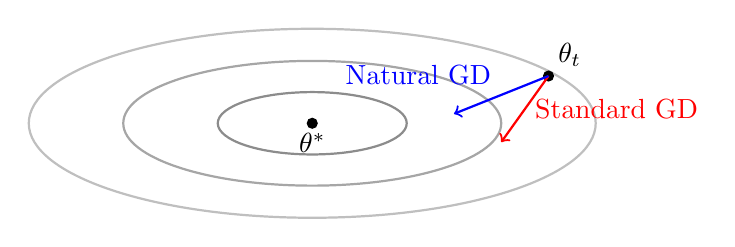
\begin{tikzpicture}[scale=1.2]
    % Contour lines for Euclidean loss
    \draw[gray!50, thick] (0,0) ellipse (3cm and 1cm);
    \draw[gray!70, thick] (0,0) ellipse (2cm and 0.66cm);
    \draw[gray!90, thick] (0,0) ellipse (1cm and 0.33cm);
    \filldraw (0,0) circle (1.5pt) node[below] {$\theta^*$};
    
    % Current parameter
    \coordinate (T) at (2.5, 0.5);
    \filldraw (T) circle (1.5pt) node[above right] {$\theta_t$};
    
    % Euclidean gradient (perpendicular to contour)
    \draw[->, red, thick] (T) -- (2.0, -0.2) node[midway, right] {Standard GD};
    
    % Natural gradient (points more towards the center due to metric correction)
    \draw[->, blue, thick] (T) -- (1.5, 0.1) node[midway, above left] {Natural GD};
\end{tikzpicture}
\caption{In parameter space, standard gradient descent follows the Euclidean normal to the loss contours, which can lead to inefficient zigzagging across valleys. Natural Gradient Descent corrects this trajectory by incorporating the Fisher Information Matrix, warping the space so that the update points more directly towards the optimum in the distribution space.}
\label{fig:ngd_vs_gd}
\end{figure}

\section{Invariance to Parameterization}

A fundamental, and arguably the most powerful, property of the natural gradient is its invariance to the choice of parameterization. Suppose we reparameterize our model using a bijective, differentiable function $\phi = g(\theta)$. The underlying probability distribution remains identical: $p_{\phi}(x) = p_{\theta}(x)$.

Let $J = \frac{\partial \theta}{\partial \phi}$ be the Jacobian of the transformation. By the multivariate chain rule, the standard gradients are related by:
\begin{equation}
    \nabla_\phi \mathcal{L} = J^\top \nabla_\theta \mathcal{L}
\end{equation}
However, the Fisher Information Matrix transforms as a covariant rank-2 tensor:
\begin{equation}
    F(\phi) = J^\top F(\theta) J
\end{equation}
Now, let us examine the natural gradient update in the new parameterization $\phi$:
\begin{align}
    \tilde{\nabla}_\phi \mathcal{L} &= F(\phi)^{-1} \nabla_\phi \mathcal{L} \nonumber \\
    &= (J^\top F(\theta) J)^{-1} (J^\top \nabla_\theta \mathcal{L}) \nonumber \\
    &= J^{-1} F(\theta)^{-1} (J^\top)^{-1} J^\top \nabla_\theta \mathcal{L} \nonumber \\
    &= J^{-1} (F(\theta)^{-1} \nabla_\theta \mathcal{L}) \nonumber \\
    &= J^{-1} \tilde{\nabla}_\theta \mathcal{L}
\end{align}
Notice that the natural gradient in $\phi$ is exactly the natural gradient in $\theta$, transformed by the inverse Jacobian. Because the parameter updates transform exactly as $d\phi \approx J^{-1} d\theta$, the update step in the distribution space is perfectly identical, regardless of whether we chose to represent our model with $\theta$ or $\phi$. Standard gradient descent explicitly lacks this crucial invariance, making its optimization trajectory an artifact of how the programmer chose to write the code.

% TikZ Figure 2: Statistical Manifold
\begin{figure}[ht]
\centering
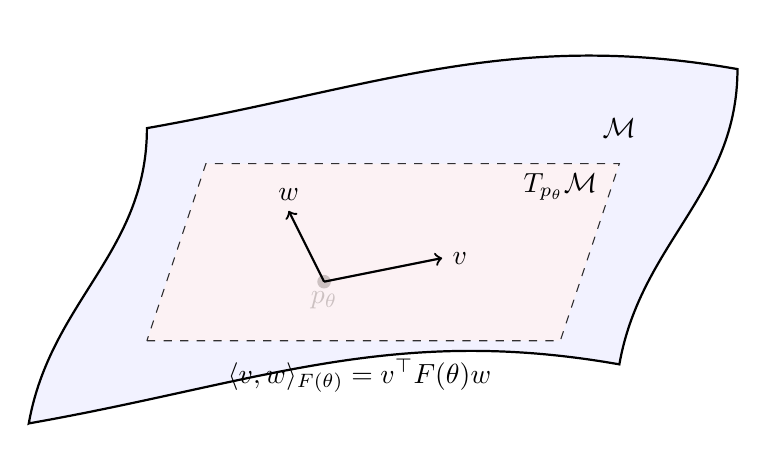
\begin{tikzpicture}[scale=1.5]
    % Manifold surface
    \draw[thick, fill=blue!5] (-2,-1) to[out=10,in=170] (3,-0.5) to[out=80,in=-90] (4,2) to[out=170,in=10] (-1,1.5) to[out=-90,in=80] cycle;
    \node at (3, 1.5) {$\mathcal{M}$};
    
    % Point p_theta
    \coordinate (P) at (0.5, 0.2);
    \filldraw (P) circle (1.5pt) node[below] {$p_{\theta}$};
    
    % Tangent space plane
    \draw[dashed, fill=red!5, opacity=0.8] (-1, -0.3) -- (2.5, -0.3) -- (3, 1.2) -- (-0.5, 1.2) -- cycle;
    \node at (2.5, 1.0) {$T_{p_\theta}\mathcal{M}$};
    
    % Vectors
    \draw[->, thick] (P) -- (1.5, 0.4) node[right] {$v$};
    \draw[->, thick] (P) -- (0.2, 0.8) node[above] {$w$};
    
    % Inner product notation
    \node at (0.8, -0.6) {$\langle v, w \rangle_{F(\theta)} = v^\top F(\theta) w$};
\end{tikzpicture}
\caption{The statistical manifold $\mathcal{M}$ of probability distributions. At any point $p_\theta$, the Fisher Information Matrix $F(\theta)$ defines an inner product on the tangent space $T_{p_\theta}\mathcal{M}$, equipping the manifold with a Riemannian metric that measures local KL divergence.}
\label{fig:statistical_manifold}
\end{figure}

\section{Numerical Example: 1D Gaussian}
Consider the task of fitting a 1D Gaussian distribution $\mathcal{N}(\mu, \sigma^2)$ to a single data point $x \sim p_{\text{data}}$ by minimizing the negative log-likelihood $\mathcal{L}$. The parameters are $\theta = [\mu, \sigma]^\top$.

The loss function is:
\begin{equation}
    \mathcal{L}(\mu, \sigma) = \frac{1}{2}\log(2\pi\sigma^2) + \frac{(x - \mu)^2}{2\sigma^2}
\end{equation}
The standard gradients are:
\begin{align}
    \frac{\partial \mathcal{L}}{\partial \mu} &= -\frac{x - \mu}{\sigma^2} \\
    \frac{\partial \mathcal{L}}{\partial \sigma} &= \frac{1}{\sigma} - \frac{(x - \mu)^2}{\sigma^3}
\end{align}
Notice the strong dependence on $\sigma$. If the variance $\sigma^2$ becomes small, the standard gradients explode dramatically, leading to severe numerical instability. Conversely, if $\sigma^2$ is large, the gradients vanish.

The Fisher Information Matrix for a 1D Gaussian parameterized by $(\mu, \sigma)$ is a diagonal matrix:
\begin{equation}
    F(\mu, \sigma) = \begin{bmatrix}
    \frac{1}{\sigma^2} & 0 \\
    0 & \frac{2}{\sigma^2}
    \end{bmatrix}
\end{equation}
The natural gradient is derived by inverting $F$ and multiplying it by the standard gradient:
\begin{align}
    \tilde{\nabla} \mathcal{L} &= F(\mu, \sigma)^{-1} \nabla \mathcal{L} \\
    &= \begin{bmatrix}
    \sigma^2 & 0 \\
    0 & \frac{\sigma^2}{2}
    \end{bmatrix}
    \begin{bmatrix}
    -\frac{x - \mu}{\sigma^2} \\
    \frac{1}{\sigma} - \frac{(x - \mu)^2}{\sigma^3}
    \end{bmatrix} \\
    &= \begin{bmatrix}
    -(x - \mu) \\
    \frac{\sigma}{2} - \frac{(x - \mu)^2}{2\sigma}
    \end{bmatrix}
\end{align}
In the natural gradient, the perilous $1/\sigma^2$ and $1/\sigma^3$ terms have been elegantly canceled out by the Fisher matrix. The update steps for both $\mu$ and $\sigma$ become highly stable, well-scaled, and completely devoid of the pathological exploding gradients seen in the Euclidean formulation. This numerical stability is a direct consequence of optimizing in the geometry of the distribution.

% 3. Horizon Box
\begin{horizon}
While Natural Gradient Descent presents a theoretically optimal way to navigate the statistical manifold, its direct application to deep learning remains a formidable computational challenge. The Fisher Information Matrix for a neural network with $d$ parameters has size $d \times d$. For modern architectures where $d \sim 10^9$, explicitly computing, storing, and inverting $F(\theta)$ is strictly intractable. 

It is conjectured that efficient approximations of the Fisher matrix, such as the Kronecker-Factored Approximate Curvature (K-FAC), capture enough of the true Riemannian geometry to yield the benefits of NGD without the debilitating $O(d^3)$ inversion cost. Future work might show that certain adaptive optimization algorithms (like Adam) or specific self-attention mechanisms inherently simulate a natural gradient step by implicitly aligning the parameter updates with the principal eigenvectors of the Fisher matrix.

An open question is whether the non-Euclidean trajectory of NGD reliably avoids the sharp, over-parameterized local minima that standard GD sometimes escapes via stochastic noise. If the information geometry of the loss landscape ultimately dictates generalization bounds, then fully realizing Natural Gradient Descent in a computationally cheap manner could fundamentally redefine the limits of large-scale model training.
\end{horizon}

% 4. Summary and Exercises
\section{Summary}
Standard gradient descent implicitly assumes a flat, Euclidean geometry in the parameter space, leading to inefficient optimization paths that are highly sensitive to how a model is parameterized. Information geometry reveals that probability distributions form a curved Riemannian manifold equipped with the Fisher Information Matrix as its metric tensor. Natural Gradient Descent corrects the standard gradient by pre-multiplying it with the inverse Fisher matrix, yielding the direction of steepest descent in terms of Kullback-Leibler divergence. This approach is intrinsically invariant to parameterization and naturally corrects for exploding or vanishing gradients induced by the geometry of the distribution, establishing a robust, theoretically rigorous foundation for optimization.

\section{Exercises}
\begin{enumerate}
    \item \textbf{Invariance Property:} Choose a new parameterization for the 1D Gaussian using precision $\rho = 1/\sigma^2$ and precision-mean $\xi = \mu/\sigma^2$. Derive the Fisher Information Matrix in terms of $(\xi, \rho)$, compute the natural gradient for this parameterization, and verify that the resulting update to the distribution is equivalent to the one derived in the chapter.
    \item \textbf{Empirical Fisher:} In practice, the true Fisher Information Matrix is often approximated using the Empirical Fisher, $F_{\text{emp}} = \frac{1}{N} \sum_{i=1}^N \nabla_\theta \log p_\theta(x_i) \nabla_\theta \log p_\theta(x_i)^\top$. Prove that $F_{\text{emp}}$ is always positive semi-definite, and discuss scenarios under which $F_{\text{emp}}$ might be a poor approximation of the true Fisher matrix.
    \item \textbf{Natural Gradient vs. Newton's Method:} Show that for a log-linear model (such as logistic regression) optimized with negative log-likelihood, the Fisher Information Matrix coincides exactly with the Hessian $H$ of the loss function. Conclude that for this specific class of models, Natural Gradient Descent is identical to Newton's Method.
\end{enumerate}

% TODO-CITE: Ensure all named results are cited.
